\documentclass{article}
\usepackage[T1]{fontenc}
\usepackage{url,color,longtable,graphicx,latexsym}

\usepackage{xcolor}
\newcommand\myworries[1]{\textcolor{red}{#1}}


\usepackage[a4paper, margin=2cm]{geometry}
\usepackage{booktabs,tabularx}
\renewcommand{\tabularxcolumn}{m}




\newcommand{\comment}[1]{
% \par\addvspace{1ex}  \noindent
% \begin{minipage}{\textwidth}\textcolor{red}{\scriptsize
%     #1} \end{minipage}
}


\newcommand{\tableentry}[3]{
\begin{minipage}{5cm}
\textbf{\small #1} 
\end{minipage}
&
\begin{minipage}{11cm}
\vskip.5em {#2} \vspace*{.5em}
% \\[.5em] {\scriptsize \textcolor{red}{#3} \vspace*{1ex} }
\end{minipage}
\\ \hline
}

\begin{document}
\subsubsection*{Article Title}
LogiKEy Workbench: Deontic Logics, Logic Combinations and Expressive
Ethical and Legal Reasoning (Isabelle/HOL Dataset)

\subsubsection*{Authors}
Christoph Benzm\"uller$^{2,1}$, Ali Farjami$^{1}$, David
Fuenmayor$^{2}$, Paul Meder$^{1}$, Xavier Parent$^{1}$, Alexander
Steen$^{1}$, Leendert van der Torre$^{1,3}$, Valeria Zahoransky$^{4}$

\subsubsection*{Affiliations}
$^{1}$University of Luxembourg, Esch sur Alzette, Luxembourg\\
$^{2}$Freie Universit\"at Berlin, Berlin, Germany \\
$^{3}$Zhejiang University, Hangzhou, China \\
$^{4}$University of Oxford, Oxford, UK\\

\subsubsection*{Corresponding author(s)}
Christoph Benzm\"uller (\url{c.benzmueller@fu-berlin.de}) \\
Xavier Parent (\url{x.parent.xaviert@gmail.com}) 

\comment{
[Firstname Lastname (email@address) – institutional email address preferred]
}


\subsubsection*{Abstract}
The LogiKEy workbench for 
%normative 
ethical and legal reasoning is presented. This workbench
simultaneously supports development, experimentation, assessment and
deployment of formal logics and ethical and legal theories at
different conceptual layers. 
More concretely, it comprises, in form of a data set (Isabelle/HOL theory
files), formal encodings of multiple deontic logics, logic
combinations, deontic paradoxes and normative theories in the
higher-order proof assistant system Isabelle/HOL.  The data was
acquired through application of the LogiKEy methodology, which
supports experimentation with different normative theories, in
different application scenarios, and which is not tied to specific
logics or logic combinations.  Our workbench consolidates
related research contributions of the authors and it may serve as a
starting point for further studies and experiments in flexible and
expressive ethical and legal reasoning. It may also support hands-on
teaching of non-trivial logic formalisms in lecture courses and
tutorials.

\comment{
[The Abstract should describe the data collection process, the analysis performed, the data, and their reuse potential. It should not provide conclusions or interpretive insights. If your article is being submitted via another Elsevier journal as a co-submission, please cite this research article in the abstract (title, or doi, and reference number only, e.g., “Title” [1]), and point the reader there for interpretation. \\
Min 100 words - Max 500 words] 
}



\subsubsection*{Keywords}
Trustworthy and responsible AI; Knowledge representation and
reasoning; Automated theorem proving; Model finding; Normative
reasoning; Normative systems; %Philosophical and ethical issues;
Semantical embedding; Higher-order logic

\comment{
[Include 4-8 keywords (or phrases) to facilitate others finding your article online. Tip: Try Google Scholar to see what terms are most common in your field. In biomedical fields, MeSH terms are a good ‘common vocabulary’ to draw from]
}



\subsubsection*{Specifications Table} 

\comment{
[Every section of this table is mandatory. Please enter information in the right-hand column and remove all the instructions]
}


\begin{longtable}{|l|l|} \hline
\tableentry
{Subject}
{Computer Science}
{[Please select one CATEGORY for your manuscript from the list available at: DIB categories.]} 

 
\tableentry
{Specific subject area}
{Artificial intelligence; Knowledge representation and reasoning; Normative reasoning}
{[Briefly describe the narrower subject area. Max 150 characters]} 


\tableentry
{Type of data}
{formal theories (.thy files) encoded in Isabelle/HOL syntax, readable
  (.png or .pdf) views of this data%,
                                %readable (pdf) views of this data
}	
{[List the type(s) of data this article describes. Simply delete from this list as appropriate:] 
Table
Image
Chart
Graph
Figure
[Any other type not listed- please specify]}


\tableentry
{How data was acquired}
{The data was acquired through manual encoding of various deontic
  logics, logic combinations, examples of contrary-to-duty paradoxes, 
  excerpts of legal texts and exemplary ethical theories utilizing the
  LogiKEy methodology \cite{J48}, which is itself based on shallow semantical
  embeddings (SSEs) \cite{J41} of logics and theories in classical higher-order
  logic. The concrete encodings were conducted in the higher-order proof
  assistant system Isabelle/HOL \cite{Isabelle}; however, they are conceptually transferable to
  other expressive reasoning systems.}	
{
[State how the data were acquired: E.g. Microscope, survey, SEM, NMR, mass spectrometry, etc. 
Instruments: E.g. hardware, software, program
Model and make of the instruments used:]}


\tableentry
{Data format}
{Raw, processed, analyzed and cleaned data. The data is provided in
  the syntax format of the Isabelle/HOL proof assistant, which has
  been used to process, analyze and verify it; the data files were
  also annotated by hand. Isabelle/HOL is freely available: \url{https://isabelle.in.tum.de}}	
{
[List your data format(s). Note, your manuscript will not be considered for publication unless you provide access to your raw data (either with article or linked to in a repository).] 
Raw
[Now simply delete from this list as appropriate:] 
Analyzed
Filtered
[Any other format not listed- please specify]}


\tableentry
{Parameters for data collection}
{One objective was to
  empirically assess the expressiveness  and proof automation
  capabilities of Isabelle/HOL and its integrated tools in normative reasoning when utilizing
  the LogiKEy methodology and the SSE
  approach. Another objective was to provide a reusable foundation for
  further experiments in expressive ethical and legal reasoning.}	
{	
[Provide a brief description of which conditions were considered for data collection. Max 400 characters]}


  \tableentry
  {Description of data collection}
  {The data were written by hand. As part of the data
  collection process it has been demonstrated
  that non-trivial, normative reasoning is
  supported in the provided framework. This in particular included
  studies of paradoxes in normative reasoning \cite{Carmo2002} and
  whether and how they can eventually be avoided.
An integral aspect of the data
  collection  
   process also has been to provide evidence for the practical
  normative reasoning performance of the various reasoning tools
  integrated with Isabelle/HOL when utilizing the LogiKEy
  approach. Useful comments were added to the data files. 
  The practical performance of the logic encodings can
  be independently assessed by users in combination with the
  Isabelle/HOL system. It has also been demonstrated how deontic
  logics can be flexible combined with other logic formalisms within the LogiKEy approach.}	
  {[Provide a brief description of how these data were collected. Max 600 characters]}


\tableentry
{Data source location}
{The data is hosted on \url{github.com}.
}	
{[Fill the available information in, and delete from this list as appropriate: 
Institution:
City/Town/Region:
Country:
Latitude and longitude (and GPS coordinates) for collected samples/data:]}


\tableentry
{Data accessibility}
{The data is accessible via  \url{logikey.org}, which redirects to
  the repository \url{https://github.com/cbenzmueller/LogiKEy} on
  \url{github.com}, where the data is hosted and maintained. The two
  subdirectories \texttt{2020-DataInBrief-Article} and
  \texttt{2020-DataInBrief-Data} are associated with this article; the
  latter contains the data set.
%Direct URL to data: \url{https://logikey.org}
}
{[State here if the data are either hosted ‘With the article’ or on a public repository. The journal does not have a strict policy but in the interest of openly sharing data we recommend hosting your data in a trusted repository. Please delete or complete as appropriate, either:]
With the article
[Or, if in a public repository:]
Repository name: [Name repository]
Data identification number: [provide number]
Direct URL to data: [e.g. https://www.data.edu.com]
[We recommend Mendeley Data if you do not have a trusted repository.]}


\tableentry
{Related research article}
{C. Benzm\"uller, X. Parent, and L. van der Torre. Designing normative
  theories of ethical and legal reasoning: LogiKEy framework, methodology, and tool support. Artificial Intelligence (to appear), 2020. Preprint: \url{https://arxiv.org/abs/1903.10187}.\\[.5em]
Further related research articles include: \cite{J46,C71,J45,C76,C77,C82}
% \\[.5em]
% $\bullet$ C. Benzm\"uller, A. Farjami, P. Meder, X. Parent, I/O Logic in HOL, Journal of Applied Logics -- IfCoLoG Journal of Logics and their Applications (Special Issue on Reasoning for Legal AI) 6 (5) 715-732, 2019. \\
% C. Benzm\"uller, A. Farjami, X. Parent, Åqvist's Dyadic Deontic Logic E in HOL, Journal of Applied Logics -- IfCoLoG Journal of Logics and their Applications (Special Issue on Reasoning for Legal AI) 6 (5) 733-755, 2019.\\
% $\bullet$ D. Fuenmayor, C. Benzm\"uller, Harnessing Higher-Order (Meta-)Logic to Represent and Reason with Complex Ethical Theories, in: A. Nayak, A. Sharma (Eds.), PRICAI 2019: Trends in Artificial Intelligence, Springer, Cham, Lecture Notes in Artificial Intelligence, volume 11670,  pp. 418-432, 2019.\\
% $\bullet$ D. Fuenmayor, C. Benzm\"uller, Mechanised Assessment of Complex Natural-Language Arguments using Expressive Logic Combinations, in: A. Herzig, A. Popescu (Eds.), Frontiers of Combining Systems, 12th International Symposium, FroCoS 2019, London, September 4-6, Springer, Cham, Lecture Notes in Artificial Intelligence, volume 11715, pp. 112-128, 2019.
}	
{	
[If your data article is related to a research article, please cite your associated research article here.
Author’s name, Title, Journal, DOI/In Press 
If your data article is not related to a research article, please delete this last row of the table]}
\end{longtable}


\subsubsection*{Value of the Data}
\begin{itemize}
\item The provided data can be reused, independent of the related
  research article(s), as a starting point for further studies and
  experiments in expressive ethical and legal
  reasoning. Moreover, it can be reused, extended and adapted to
  support also other various other application directions, including, e.g.,~the study of deontic modality and quantifiers in linguistics.

\item The data collection is beneficial for research and application
  in a range of areas, including but not limited to: machine ethics
  (ethico-legal governor systems), explainable and trustworthy AI,
  regulatory technologies, argumentation, natural language semantics. To that end the data includes reusable SSEs
  of a portfolio of deontic logics, logic combinations, paradoxes in
  normative reasoning and ethical theories in classical higher-order
  logic (HOL), aka Church's type theory \cite{J43}, interpretable in
  the Isabelle/HOL proof assistant system \cite{Isabelle}. The data
  set may also be used to support the teaching of expressive,
  classical and non-classical logic
  formalisms and their combinations in lecture courses and tutorials.

\item To reuse the data interested researchers, 
  students and practitioners only 
  need to download the provided data files, include them in their
  formalization projects and suitably extend or adapt them. For
  example, the contributed data includes a sample encoding of selected
  statements from the GDPR (General Data Protection Regulation) and an
  encoding of Gewirth's ethical argument and principle, known as the
  Principle of Generic Consistency (PGC) \cite{GewirthRM}, in a suitable extension of
  higher-order deontic logic. These are two examples in the area of
  knowledge representation and reasoning with an emphasis on
  regulatory and ethical aspects. They can be reused as a starting
  point for the encoding and automated solution of similar
  ethico-legal theories.

\item  The data set advances the state of the art in deontic logic \cite{gabbay2013} as follows. Sixty years after Von Wright's invention of deontic logic, the
  question has always been how deontic logics and normative theories
  can be used in computer science applications. The LogiKEy 
  workbench and associated methodology addresses this challenge; it has the potential to revolutionize the
  area of deontic logic itself.


\item The data set is useful also for stimulation of
  cross-fertilization effects between different research communities including
  the deontic logics  and normative reasoning communities,
  the area of higher-order logics, and the area of  interactive
  and automated theorem proving with its various sub-communities targeting
  very different logic formalisms.

\item The presented encodings put a particular emphasis on the
  modeling of (regulative) norms. We agree with, e.g., Jones and
  Sergot \cite{Jones1992-JONDLI} that deontic logic is needed when it is necessary to make
  explicit, and then reason about, the distinction between what ought
  to be the case and what is the case. Furthermore, the adequate
  handling of the deontic paradoxes (like in particular Chisholm's paradox of contrary-to-duty obligation, which deals with norm violation)
  posed a core challenge for knowledge representation
  frameworks. This problem motivated the design of deontic logics (and logic combinations) more sophisticated and finer-grained than the traditional ones, like modal logic. These frameworks are automatized for the first time.  It is demonstrated that a computer or a machine can reason about norm violation during run-time.  

%The work of those interested in automated reasoning for
%  normative reasoning usually goes on as if the intricacies of
%  contrary-to-duty norms had never been heard of.

\end{itemize}

\comment{
[Provide 3-6 bullet points explaining why these data are of value to the scientific community. Bullet points 1-3 must specifically answer the question in red next to the bullet point, but do not include the question itself in your answer (i.e.,for the first bullet, you should explain why these data are useful but delete the “Why are these data useful?” question text itself). You may provide up to 3 additional bullet points to outline the value of these data. Please keep points brief.
·	Why are these data useful?
·	Who can benefit from these data?
·	How can these data be used for further insights and development of experiments?
·	 What is the additional value of these data?
·	…
·	…]
}

\subsubsection*{Data Description}
The data is provided in form of Isabelle/HOL source files, which are
hosted at \url{logikey.org}. The individual data files belong to different
categories. 


% \begin{figure}[t]
%  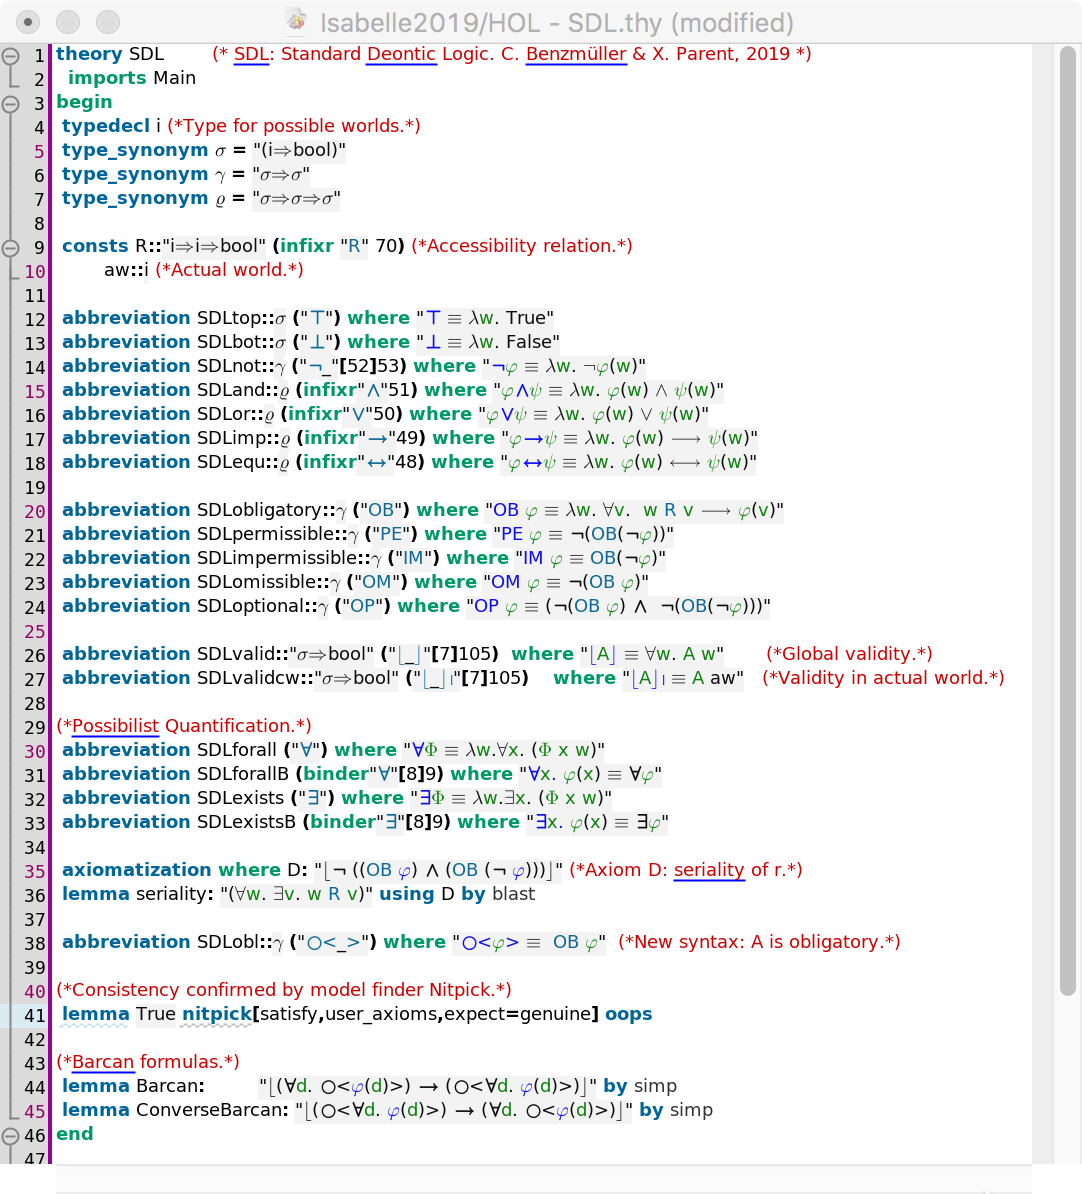
\includegraphics[width=\textwidth]{SDL.png}
% \caption{Data file \textsf{\small \detokenize{SDL.thy} contributes an
%     SSE of a quantified extension of SDL in HOL \label{fig:SDL}}}
% \end{figure}

Contributed data files in category I are listed in
Table~\ref{table:DeonticLogics}. They provide encodings of SSEs, and
associated tests, of various deontic logics in meta-logic HOL.  A category I 
example file is displayed in Figs.~\ref{fig:CJ_DDLplus1}--\ref{fig:CJ_DDLplus2}; this
data file contains (an extension of) the SSE of 
 dyadic deontic logic (DDL) by Carmo and Jones \cite{CJ13} in HOL and
 studies, resp.~verifies, its properties.

\begin{figure}[ht!]
 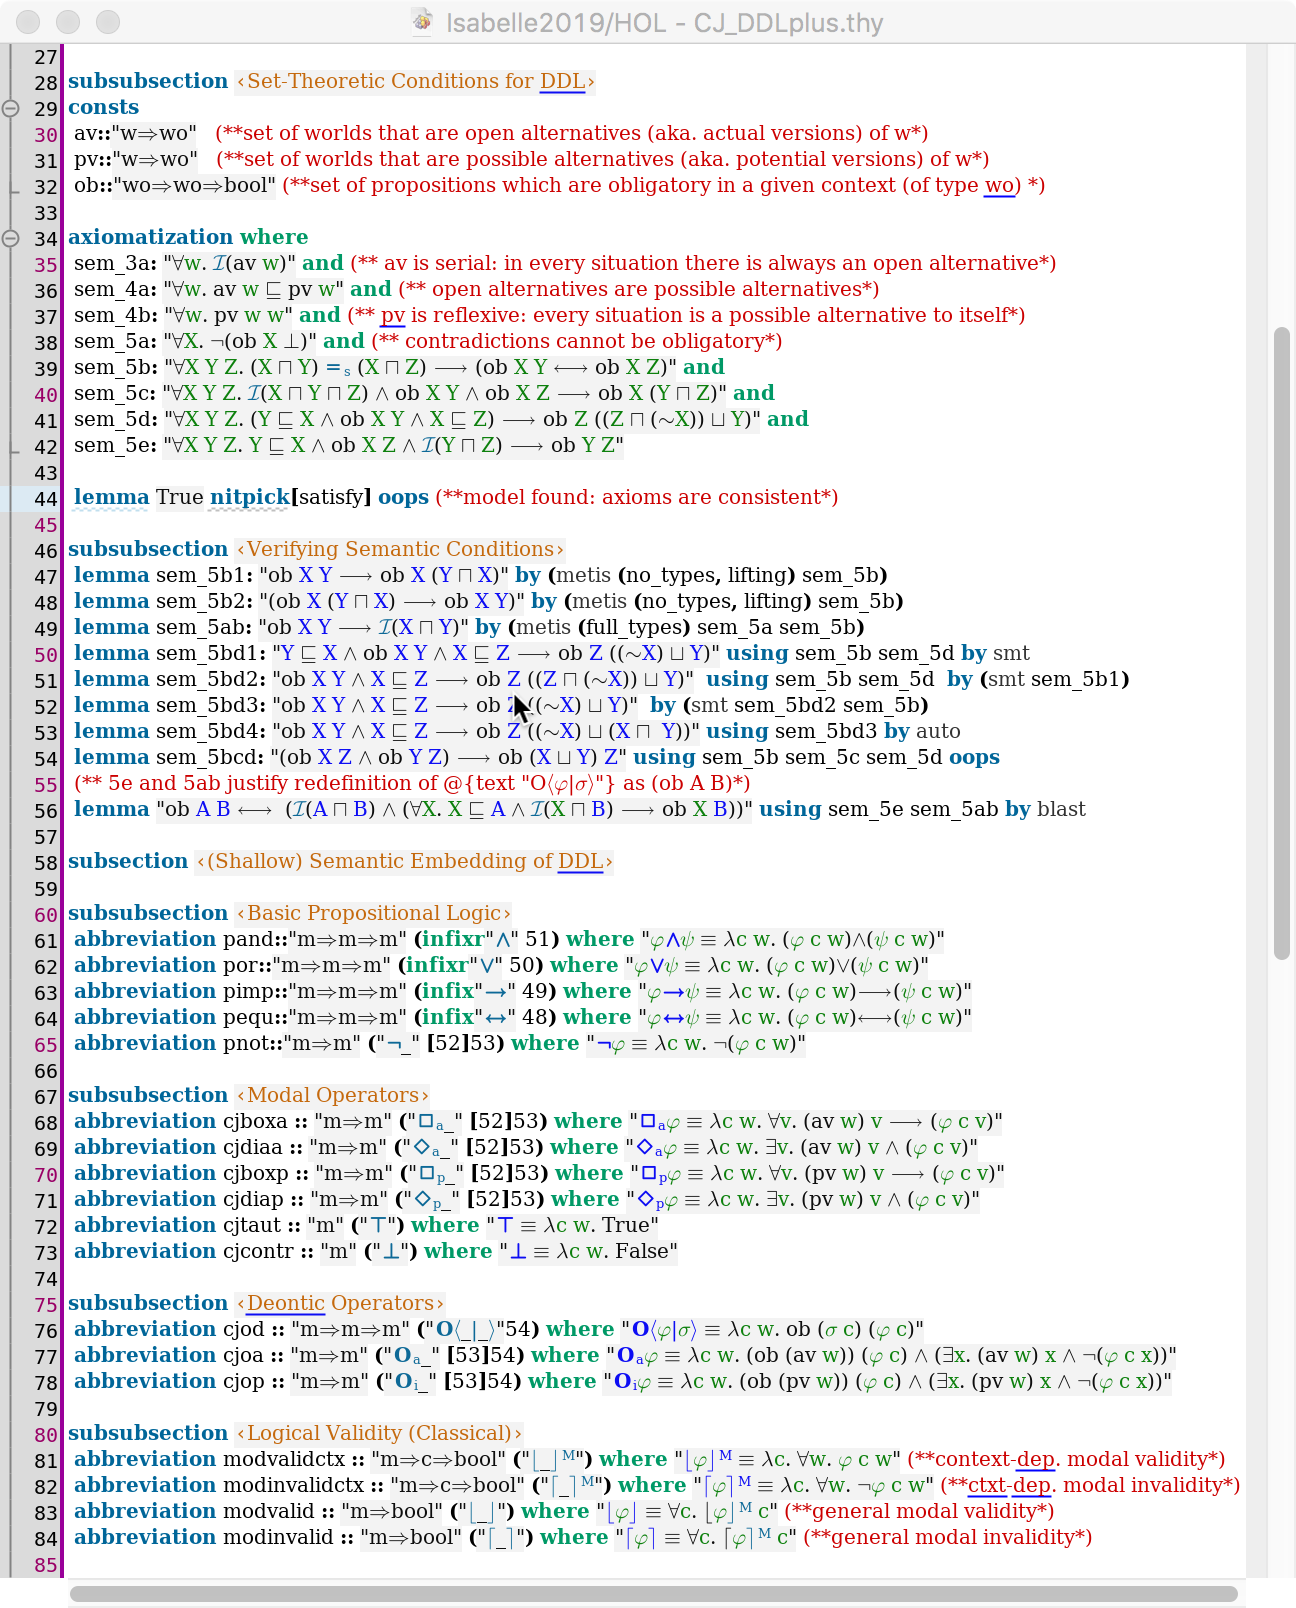
\includegraphics[width=\textwidth]{CJ_DDLplus1.png}
\caption{Data file \textsf{\small \detokenize{CJ_DDLplus.thy}; in
    lines 29--85 the SSE of the DDL by  Carmo and Jones \cite{CJ13} in HOL is presented \label{fig:CJ_DDLplus1}}}
\end{figure}



\begin{figure}[ht!]
 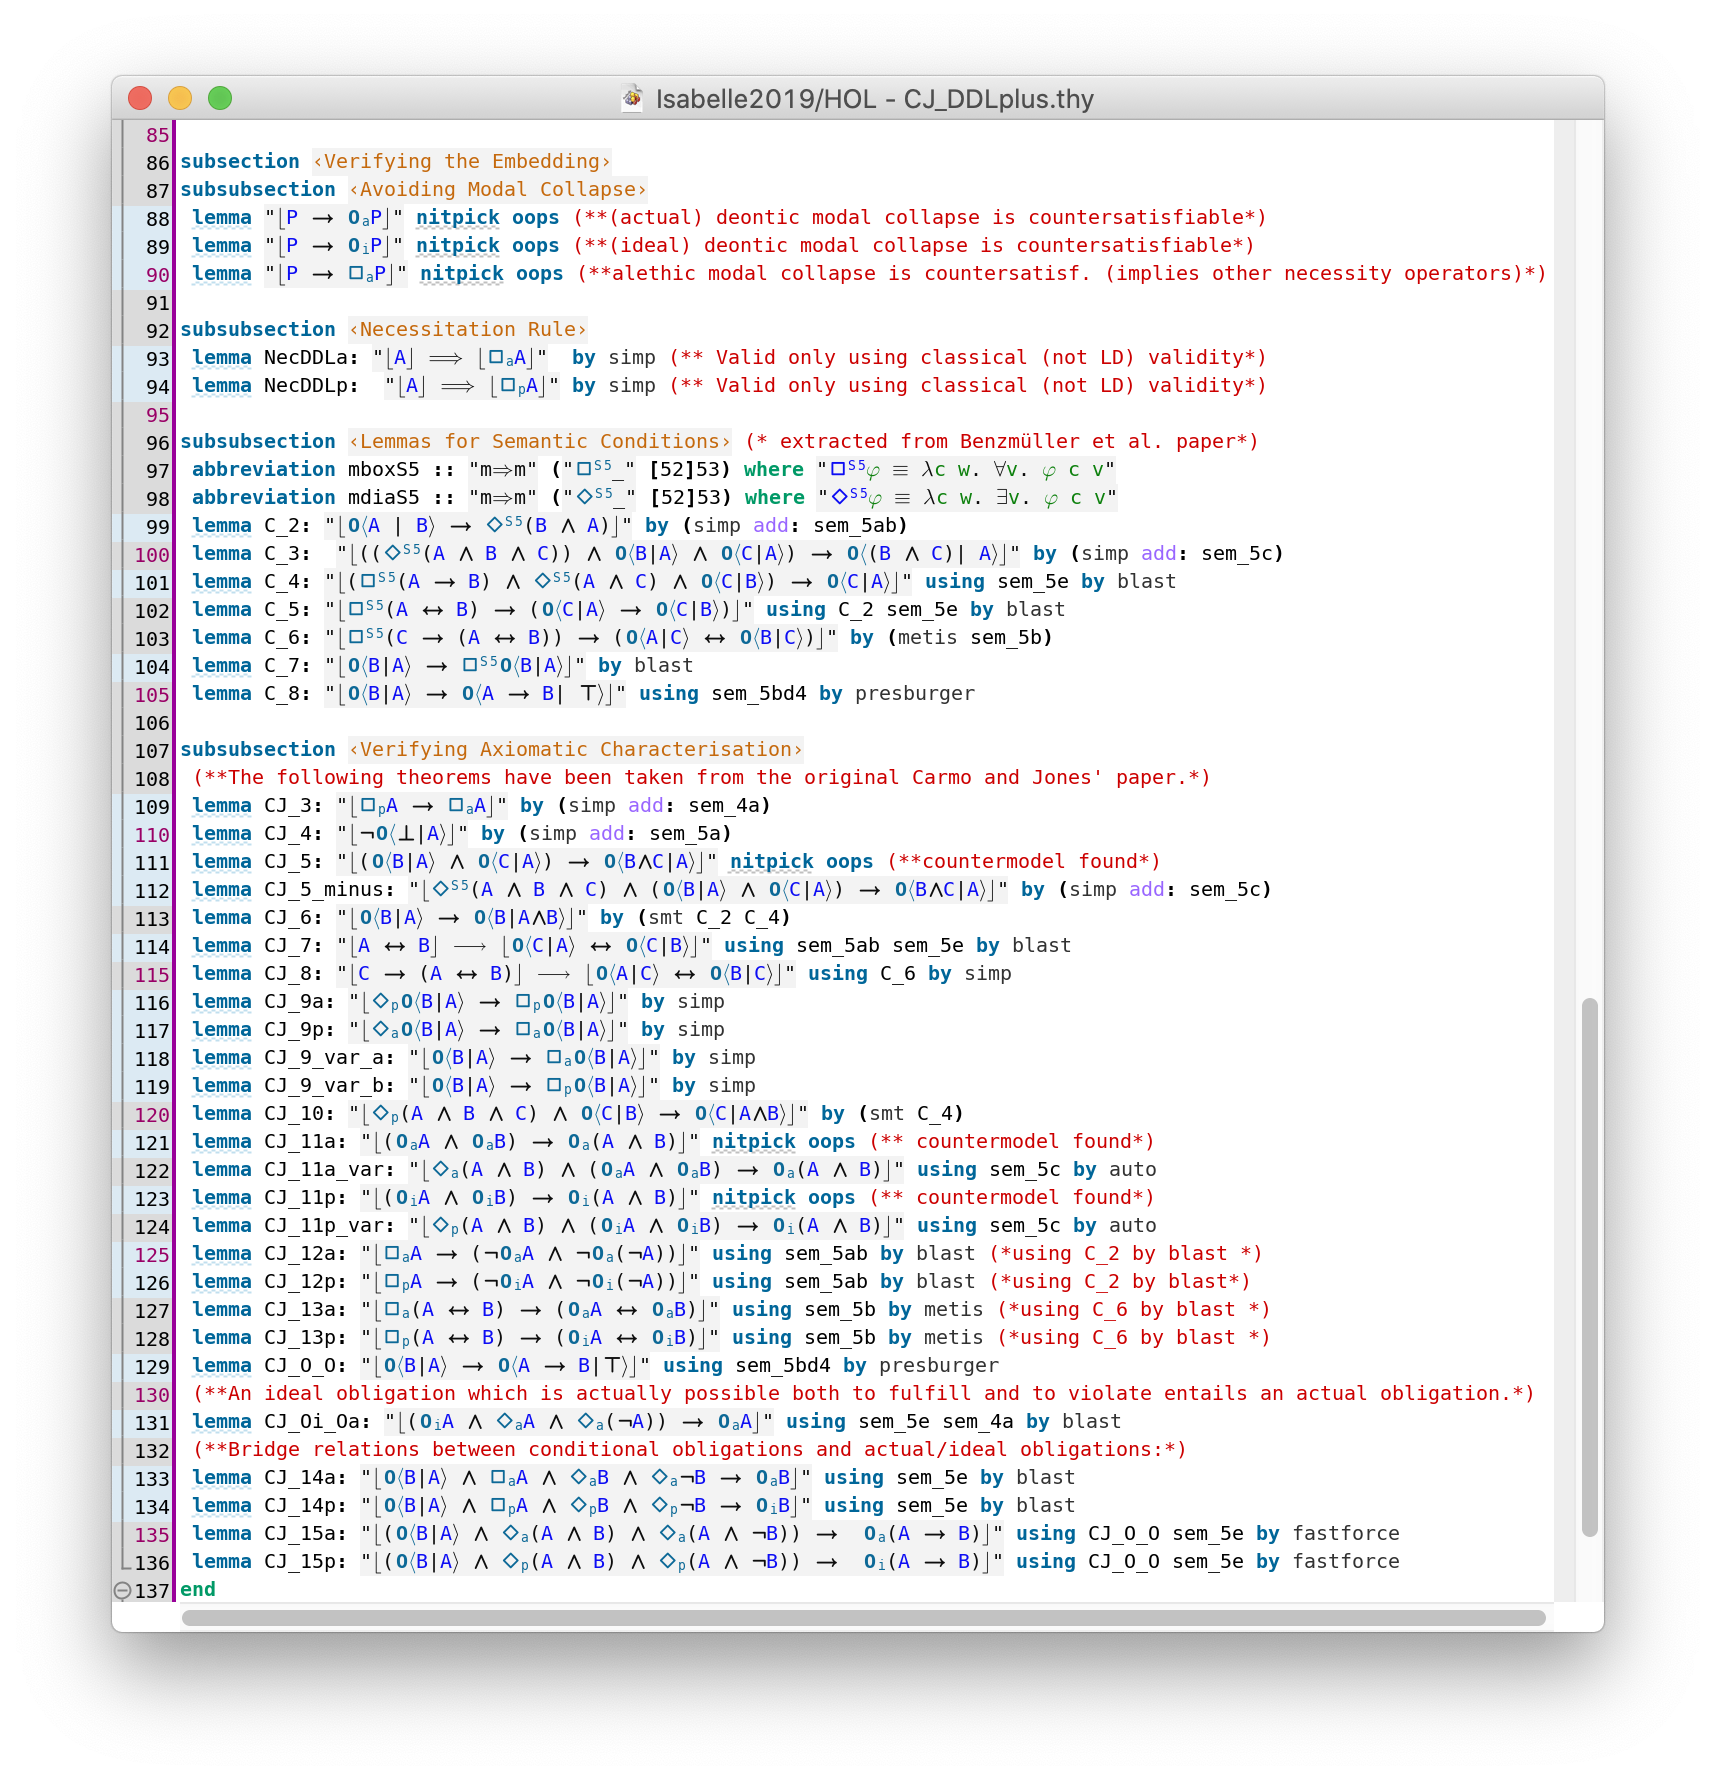
\includegraphics[width=\textwidth]{CJ_DDLplus2.png}
\caption{Data file \textsf{\small \detokenize{CJ_DDLplus.thy}; in
    lines 87--137 lemmata from Carmo and Jones's paper \cite{CJ13} are
    proved \label{fig:CJ_DDLplus2}}}
\end{figure}


\setcounter{table}{0}
\begin{table}[htp!]
\caption{Category I data files --- deontic logics, extensions of
  deontic logics and logic combinations \label{table:DeonticLogics}}
\begin{tabularx}{\textwidth}{ccc*{1}{>{\raggedright\arraybackslash}X}}
  \toprule
  File & Dependency & Reading & Description \\
  \midrule
  \textsf{\small SDL.thy} 
       & \textsf{\small Main.thy} 
                    & \cite{J23,ddl:C80}  
                              & % Provides a consistent SSE of SDL in
                                % HOL; see Fig.~\ref{fig:SDL}. An unary deontic operator is
                                % defined (lines 20 and 38).
                                % The D axiom is postulated (line 35) and correspondence to seriality of the
                                % accessibility is proved (line 38). The added
                                % first-order and higher-order
                                % quantifiers (lines 30--33) are constant domain
                                % (possibilist notion of quantification). This is verified by proving
                                % the Barcan formula and its
                                % converse. \\
                                Provides a SSE of standard
  deontic logic (SDL) in
                                HOL. An unary deontic operator is
                                defined.
                                The D axiom is postulated and correspondence to seriality of the
                                accessibility is proved. The added
                                first-order and higher-order
                                quantifiers are constant domain
                                (possibilist notion of quantification). This is verified by proving
                                the Barcan formula and its converse. \\
  \midrule
  \textsf{\small \detokenize{CJ_DDL.thy}}
       & \textsf{\small Main.thy} 
                    & \cite{C71}  
                              &  Provides a SSE of a dyadic deontic
                                logic (DDL) by Carmo
                                and Jones \cite{Carmo2002} in HOL.  Different modal
                                operators are introduced: dyadic deontic
                                obligation, monadic deontic operator for
                                actual obligation, monadic
                                deontic operator for primary
                                obligation,
                                and further alethic modalities.
                                Moreover, constant domain first-order and higher-order
                                quantifiers are added.\\
                                % Provides a consistent SSE of a
                                % dyadic deontic
                                % logic (DDL) by Carmo
                                % and Jones \cite{CJ13} in HOL; see
                                % Fig.~\ref{fig:DDL}.  Different modal
                                % operators are introduced: dyadic
                                % deontic
                                % obligation (line 33; see also line
                                % 49), monadic deontic operator for
                                % actual obligation (line 34), monadic
                                % deontic operator for primary
                                % obligation (line 35),
                                % and further alethic modalities
                                % (lines
                                % 27--32).
                                % Moreover, constant domain
                                % first-order
                                % and higher-order
                                % quantifiers are added (lines
                                % 40-43).\\
  \midrule
  \textsf{\small \detokenize{CJ_DDL_Tests.thy}}
       & \textsf{\small \detokenize{CJ_DDL.thy}}
                    & \cite{C71}  
                              & Contains
                                soundness and proof automation tests for the
                                embedding of DDL in HOL given in
                                \textsf{\small \detokenize{CJ_DDL.thy}}. For example,
                                the monadic modal operators $\Box$,
                                $\Box_p$ and $\Box_a$ are  identified
                                as S5, KT and KD modalities,
                                respectively. Relevant lemmata from the original work
                                of Carmo and Jones are
                                automated. \\
                               % This file, see Fig.~\ref{fig:DDL_Tests}, contains
                                % soundness and proof automation tests for the
                                % embedding of DDL in HOL given in
                                %  \textsf{\small CJ_DDL.thy}. For example,
                                %   the monadic modal operators $\Box$,
                                % $\Box_p$ and $\Box_a$ are  identified
                                % in lines 11--25
                                % as S5, KT and KD modalities,
                                % respectively. Relevant lemmata (see
                                % the entries with name prefixes
                                % $C\_1$--$C\_15$) from the original work
                                % of Carmo and Jones \cite{CJ13} are
                                % automated, except for the two lemmata
                                % $C\_3$ and $C\_8$ which are
                                % open benchmark problems for theorem
                                % provers, and which so far
                                % can only be proved interactively (not given here).\\
  \midrule
  \textsf{\small E.thy} 
       & \textsf{\small Main.thy} 
                    & \cite{J45},\cite[Fig.6]{J48}  
                              & Provides a SSE of a quantified extension of
                                Aqvist's System E in HOL. The file also
                                runs a number of reasoning tasks (validity checking, refutation, correspondence theory).\\
  \midrule
  \textsf{\small \detokenize{Lewis_DDL.thy}}
       & \textsf{\small Main.thy} 
                    & \cite{ddl:L73}  
                              & Provides a SSE of Lewis's DDL.
                                The file
                                runs a number of reasoning tasks
                                (validity checking, refutation,
                                correspondence theory). The
                                relationship with \AA qvist's dyadic
                                deontic operator is also studied.\\
 \midrule
  \textsf{\small \detokenize{IOL_out2.thy}}
       & \textsf{\small Main.thy} 
                    & \cite{J46}  
                              & Provides a SSE of a quantified extension of
                                IO logic (out$_2$) \cite{DBLP:journals/jphil/MakinsonT00,textbook18}. The file also
                                contains an analysis of a benchmark example discussed in the literature on moral luck. \\
  \midrule
  \textsf{\small \detokenize{IO_out2_STIT.thy}}
       & \textsf{\small Main.thy} 
                    & \cite{J46,MederMasters}  
                              & Provides a SSE of a quantified extension of
                                IO logic (out$_2$) \cite{DBLP:journals/jphil/MakinsonT00,textbook18} and elements of STIT logics \cite{horty} in HOL. The file also
                                contains proof automation tests and
                                soundness checks. \\
  \midrule
  \textsf{\small \detokenize{CJ_DDLplus.thy}}
       & \textsf{\small  Main.thy} 
                    & \cite{C76,C77}
                              & A modification of the SSE developed in
                                file \textsf{\small \detokenize{CJ_DDL.thy}} is
                                presented; see
                                Figs.~\ref{fig:CJ_DDLplus1}
                                and~\ref{fig:CJ_DDLplus2}. This theory provides the starting point
                                for an extension of a higher-order
                                variant of DDL into a
                                two-dimensional semantics as
                                originally presented by Kaplan
                                for his logic of demonstratives~\cite{Kaplan1979,Kaplan1989}. The logic extension is
                                completed in file \textsf{\small
                                \detokenize{Extended_CJ_DDL.thy}}. The
                                displayed lines in Fig.~\ref{fig:CJ_DDLplus2} show
                                automations of various lemmata
                                from the original paper of Carmo
                                and Jones \cite{CJ13}, where they were
                                proved manually with pen and paper. \\
  \midrule
  \textsf{\small \detokenize{Extended_CJ_DDL.thy}}
       & \textsf{\small \detokenize{CJ_DDLplus.thy}}
                    & \cite{C76,C77}
                              & Contains a further extension and
                                combination of the
                                higher-order DDL encoded in file
                                \textsf{\small
                                \detokenize{CJ_DDLplus.thy}} with
                                relevant parts (for the work presented
                                in the related research article
                                \cite{J48}) of Kaplan's logic of demonstratives (LD)~\cite{Kaplan1979,Kaplan1989}.\\
  \bottomrule
\end{tabularx}
\end{table}



Contributed data files in category II are listed in
Table~\ref{table:Paradoxes}. They study paradoxes and smaller examples
of normative reasoning. An example is displayed in
Fig.~\ref{fig:Chisholm_SDL}, which presents an analysis of Chisholm's
paradox of contrary-to-duty obligation \cite{c63} in Standard Deontic Logic (SDL). The known fact that SDL cannot handle CTD scenarios is confirmed by the computer. 


% \begin{figure}[ht!]
%  \includegraphics[width=\textwidth]{DDL_Tests.png}
% \caption{Data file \textsf{\small \detokenize{CJ_DDL_Tests.thy} \label{fig:DDL_Tests}}}
% \end{figure}

\begin{table}[ht!]
\caption{Category II data files: paradoxes and examples of normative reasoning \label{table:Paradoxes}}
\begin{tabularx}{\textwidth}{ccc*{1}{>{\raggedright\arraybackslash}X}}
  \toprule
  File & Dependency & Reading & Description \\
  \midrule
  \textsf{\small \detokenize{Chisholm_SDL.thy}}
       & \textsf{\small SDL.thy} 
                    & \cite{textbook18}
                              &  The well-known analysis of Chisholm's contrary-to-duty paradox
                                in SDL is automated. The formalization uses both the wide-scope interpretation of conditional ``ought" and the narrow-scope one; see Fig.~\ref{fig:Chisholm_SDL}. \\
  \midrule
  \textsf{\small \detokenize{Chisholm_CJ_DDL_Monadic.thy}}
       & \textsf{\small \detokenize{CJ_DDL.thy}} 
                    &  --
                              &  Contains a study analogous to \textsf{\small
                                \detokenize{Chisholm_SDL.thy}} for 
                                monadic obligation in DDL. \\
  \midrule
  \textsf{\small \detokenize{Chisholm_CJ_DDL_Dyadic.thy}}
       & \textsf{\small \detokenize{CJ_DDL.thy}}
                    & --
                              &  Contains a study analogous to \textsf{\small
                                \detokenize{Chisholm_SDL.thy}} for 
                                dyadic  obligation in DDL. \\
  \midrule
  \textsf{\small \detokenize{Chisholm_E.thy}}
       & \textsf{\small \detokenize{CJ_DDL.thy}}
                    & --
                              &  Contains a study analogous to \textsf{\small
                                \detokenize{Chisholm_SDL.thy}} for 
                                deontic logic E. \\
  \midrule
  \textsf{\small \detokenize{IO_Experiments}}
       & \textsf{\small \detokenize{IO_out2_STIT}}
                    & \cite{MederMasters} 
                              &  Contains a study of different paradoxes from the literature in IO
                                logic (out$_2$); the file 
                                imports \textsf{\small \detokenize{IO_out2_STIT}}.\\
  \bottomrule
\end{tabularx}
\vskip1em
\end{table}

\begin{figure}[ht!]
 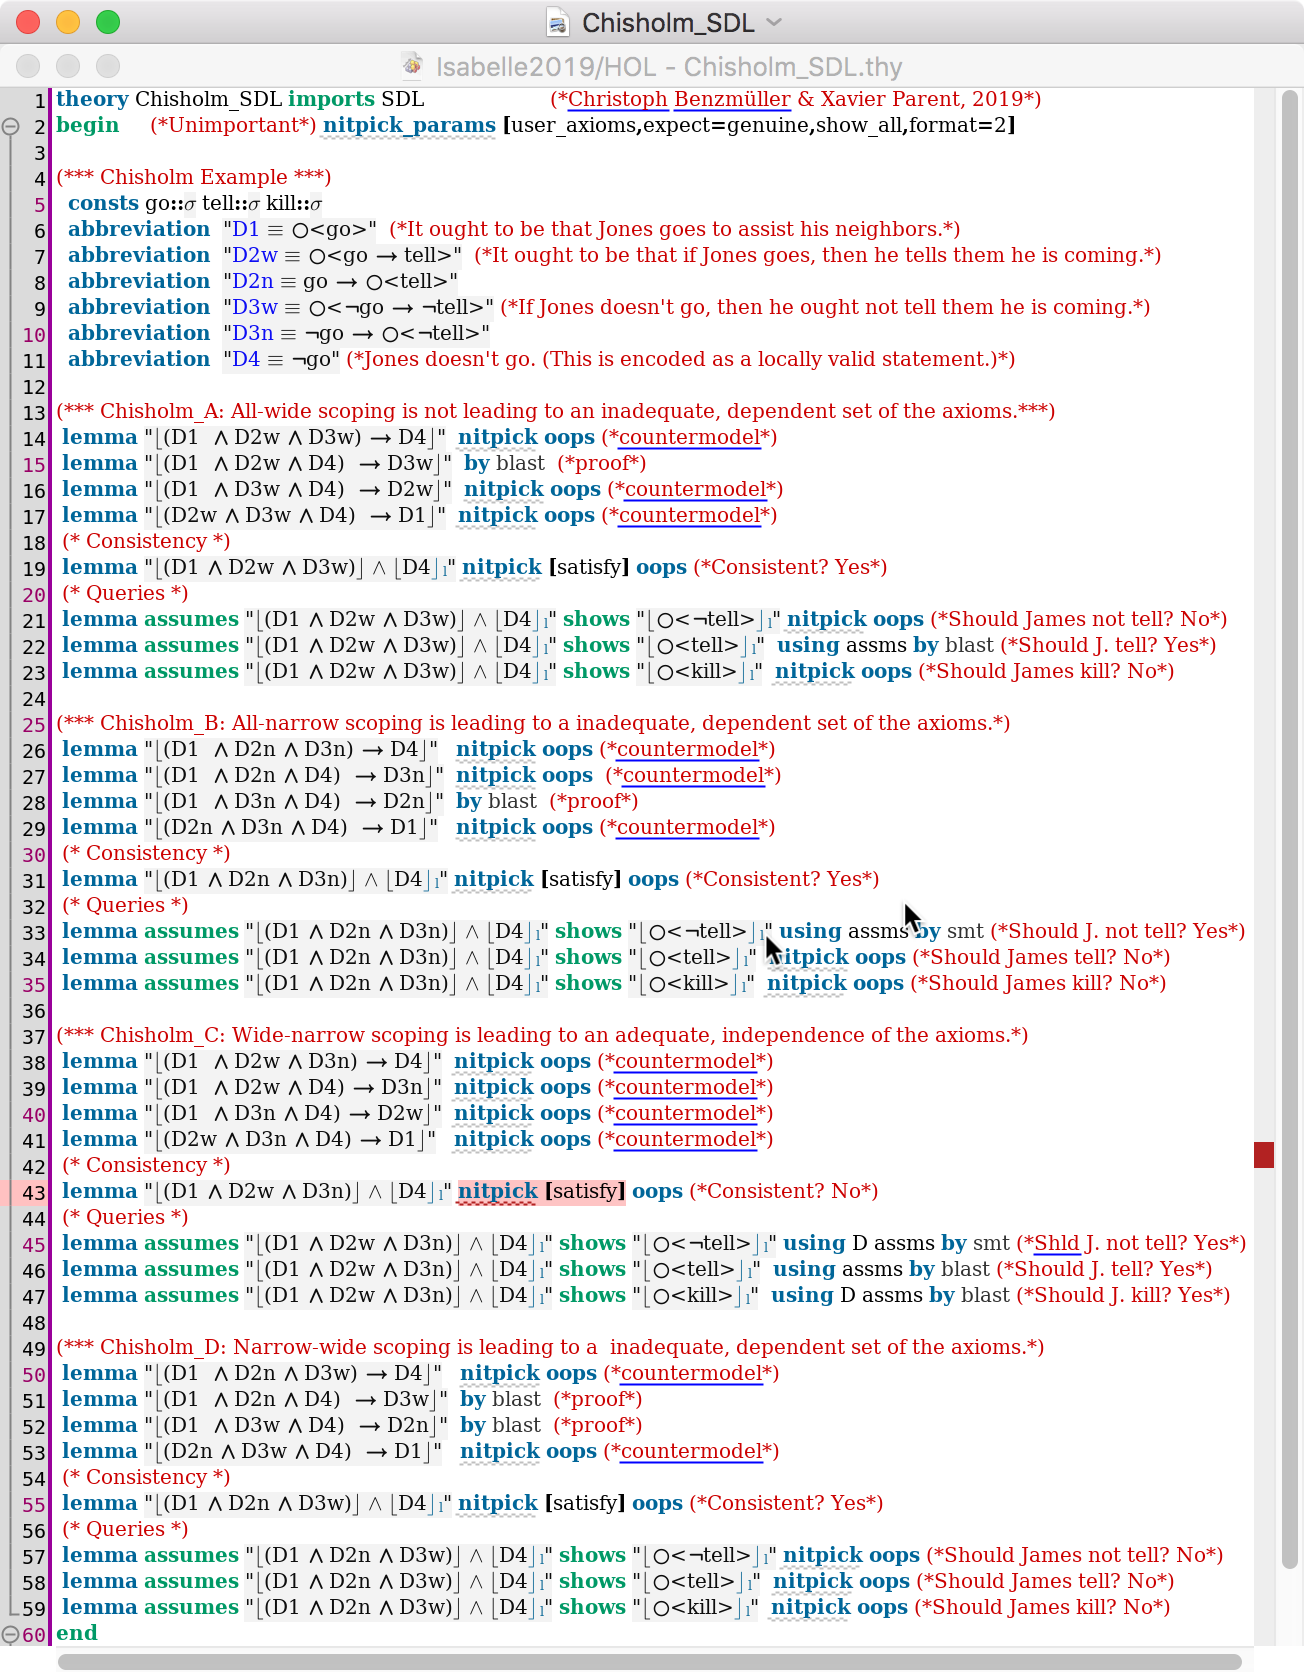
\includegraphics[width=\textwidth]{Chisholm_SDL.png}
\caption{Data file \textsf{\small \detokenize{Chisholm_SDL.thy}
    studies 
    Chisholm's paradox in combination with 
    wide-narrow scoping issues \label{fig:Chisholm_SDL}}}
\end{figure}

Contributed data files in category III are listed in
Table~\ref{table:Theories}. They provide an encoding of (excerpt of)
legal and ethical theories and arguments formalized using the deontic logics as
provided in category I files and further examined in the category II
files.

In addition to data listed in
Tables~\ref{table:DeonticLogics}---\ref{table:Theories} the data set
provided at \url{logikey.org} also includes the following:
\begin{itemize}
\item Subdirectory \url{2020-DataInBrief-Data/Course-Material-1} contains Isabelle/HOL data files stemming from a
  lecture course on deontic logic at University of Luxembourg based on \cite{textbook18}.
\item Subdirectory \url{2020-DataInBrief-Data/Climate-Engineering} contains Isabelle/HOL data files related to the
  formalization and assessment  \cite{C82}  of selected arguments in climate engineering.
\item  Subdirectory \url{2020-DataInBrief-Data/US-Constitution-Loophole} contains Isabelle/HOL data files related to a 
  formalization and assessment  \cite{zahoransky19} of Kurt G\"odel's claim that the US Constitution contains a
  loophole for establishing a dictatorship.
\item  Subdirectory \url{2020-DataInBrief-Data/WiseMenPuzzle} contains Isabelle/HOL data files related to a 
  formalization and study \cite{J41} of the well known Wise Men
  Puzzle; this data set, which has been published before~\cite{J44}, is
  included here to make it better available for 
  \url{logikey.org} users.
\end{itemize}

Further related data sets, including
  selected formalisations in computational metaphysics
  (cf.~\cite{J41,J47} and the references therein), will be added to 
   \url{logikey.org} as we think fit.

% There are related works in normative reasoning (see
% e.g.~Maja?,}) and in computational metaphysic
% (see e.g.~\cite{J47} and the references therein) that have 
% employed the LogiKEy methodology, but which, for various reasons, are not
% included in our data set.

  
\begin{table}[ht!]
\caption{Category III data files: (excerpts of) legal and ethical
  theories and arguments \label{table:Theories}}
\begin{tabularx}{\textwidth}{ccc*{1}{>{\raggedright\arraybackslash}X}}
  \toprule
  File & Dependency & Reading & Description \\
  \midrule
  \textsf{\small \detokenize{GDPR_SDL.thy}}
       & \textsf{\small SDL.thy} 
                    & \cite[Fig. 7]{J48}
                              &  Contains a modeling of selected statements from the GDPR in
                                first-order SDL. It is confirmed by automated means that first-order SDL cannot handle  
                                contrary-to-duty scenarios.\\
  \midrule
  \textsf{\small \detokenize{GDPR_CJ_DDL.thy}}
       & \textsf{\small \detokenize{CJ_DDL.thy}} 
                    &  ---
                              &  Contains a modeling of selected statements from the GDPR in
                                first-order DDL. It is confirmed by automated means that the logic can handle  
                                contrary-to-duty scenarios. The problems identified in \textsf{\small
                                \detokenize{GDPR_SDL.thy}}, i.e., inconsistency and explosion, are
                                avoided. The reasoners return ``intuitive'' answers to queries. \\
  \midrule
  \textsf{\small \detokenize{GDPR_E.thy}}
       & \textsf{\small E.thy} 
                    & \cite[Fig. 8]{J48}
                              &  Contains a modeling of selected statements from the GDPR in
                                a first-order extension of logic E. It is confirmed by automated means that the logic can handle  
                                contrary-to-duty scenarios, and does not face the problems  identified in \textsf{\small
                                \detokenize{GDPR_SDL.thy}}, i.e., inconsistency and explosion. \\
  \midrule
  \textsf{\small \detokenize{GewirthArgument.thy}}
       & \textsf{\small \detokenize{Extended_CJ_DDL.thy}}.
                    & \begin{minipage}{2cm} \cite{C77,C76}, \\
                      \cite[Fig. 10]{J48} \end{minipage}
                              & Contains a formalization and partial automation of Gewirth's
                                supporting argument for his \textit{Principle of Generic
                                Consistency}. This principle
                                constitutes, loosely speaking, an emendation of the
                                \emph{Golden Rule}, i.e., the
                                principle of treating others as one's
                                self would wish to be
                                treated. Gewirth's argument and theory
                                is
                                assessed, emended (minor corrections)
                                and verified. \\
  \bottomrule
\end{tabularx}
\vskip1em
\end{table}



\comment{
[Describe your data and remember to refer to each data file (i.e., figure 1, figure 2, table 1, dataset, raw data, supplemental data, etc.) that are included in this article. Please provide a clear description of each file – do not simply list them. No insight, interpretation, background or conclusions should be included in this section. Min word 150, no maximum]
}

\subsubsection*{Experimental Design, Materials, and Methods}

The data was acquired through manual encodings of logics, theories and
arguments in the
Isabelle/HOL \cite{Isabelle} proof assistant system. The modeling
process was following the LogiKEy methodology depicted in
Fig.~\ref{fig:LogiKEy}. This methodology supports formalization
projects in the area of ethical and legal reasoning at different
layers of abstraction. This methodology is briefly explained below at hand of
selected examples from our contributed data set; we address all three
different layers and discuss examples.\footnote{For a general
description of the LogiKEy framework, methodology and tool support see
the related research article~\cite{J48}.}

\begin{description}
\item{Layer L1 example development (files \textsf{\small
      \detokenize{CJ_DDL.thy}} and \textsf{\small
      \detokenize{CJ_DDL_Tests.thy}}):} File \textsf{\small
    \detokenize{CJ_DDL.thy}} contains the encoding (of a quantified
  extension) of the DDL of Carmo and Jones in
  HOL. This encoding of DDL in HOL is exemplary for \textit{Layer L1}
  developments in LogiKEy. First, the desired object \textit{logic}
  was selected (Step~1); Carmo and Jones's DDL in the given case. A \textit{semantics}
  (Step 2) for this object logic was sought and found in the original
  papers by Carmo and Jones \cite{Carmo2002}; such a mathematical
  description of a semantics, a neighborhood semantics in the given
  case, constitutes the ideal starting point for the definition of a
  SSE of the object logic in HOL, which in turn enables its
  \textit{automation} (Step 3) with off-the-shelf reasoning tools for
  HOL. The automation of DDL was subsequently assessed (Step 4) with
  automated theorem provers and model finders integrated with
  Isabelle/HOL. Then, by pen and paper means on a theoretical level,
  the \textit{faithfulness} (Step 4) of the embedding of DDL in HOL
  was studied and proved; this proof has been published
  \cite{C71,R63}. Furthermore, \textit{implications} of the embedding
  of DDL in HOL were studied (Step 5); see for example the additional
  theorems in file \textsf{\small \detokenize{CJ_DDL_Tests.thy}} and
  the analysis of contrary-to-duty scenarios conducted in files
  \textsf{\small \detokenize{Chisholm_DDL_Monadic.thy}} and
  \textsf{\small \detokenize{Chisholm_DDL_Dyadic.thy}}. Since the DDL
  of Carmo and Jones has not been automated before with other systems
  or approaches, there are no \textit{benchmarks} (Step 7) available
  that we could use to properly assess and compare the competitiveness
  of our solution. The publication of this data set can be seen as a
  first step towards the built-up and \textit{contribution} (Step 8)
  of such a benchmark suite to the community; future work includes the
  conversion of our Isabelle/HOL encodings into TPTP THF format
  \cite{J22}, so that they can be used as benchmark problems in the yearly CASC
  world-championship competitions
  \cite{DBLP:journals/aim/Sutcliffe16}.

\item{Layer L2 example development (file \textsf{\small
      \detokenize{GDPR_CJ_DDL.thy}}):} In file \textsf{\small
    \detokenize{GDPR_CJ_DDL.thy}} we \textit{selected} (Step 1)
  statements from the General Data Protection Regulation (GDPR) for
  formalisation. The \textit{analysis} (Step 2) of these statements
  revealed that obligation aspects in the context of data processing
  needed to be addressed. Natural language phrases in the
  studied parts of the GDPR indeed contains occurrences of the deontic
  modalities. This motivated the choice of a suitable deontic
  \textit{logic} (Step 3), such as DDL, for the formal encoding of
  these challenging aspects. In the given case it also  became apparent that
  a propositional encoding would hardly suffice in practical
  applications, so the selected deontic logic DDL needed to be
  \textit{combined with}, respectively extended by, a notion of
  quantification, which led to the addition of quantifiers to the file
  \textsf{\small \detokenize{CJ_DDL.thy}}. Subsequently the two GDPR
  articles were \textit{formalized} (Step 4) using logical connectives
  as provided in the imported file \textsf{\small
    \detokenize{CJ_DDL.thy}}, and then some \textit{exploration} (Step
  5) and assessment studies were conducted. This included the analysis of the 
  contrary-to-duty scenario as reported in related research articles
  \cite{J48,C71}. With our data set we \textit{contribute} (Step 6)
  this work to the wider research community and enable its reuse.

\item{Layer L3 example development:}  Layer L3 example developments
  have just started. The idea is to populate regulatory governor
  architectures \cite{J48}
  with ethical and legal theories from Layer L2, so that reasoning with the
  theories can be utilized to explain and control the behaviour of
  (autonomous) AI systems. To realize such applications it is required
  to \textit{select} (Step 1) some ethical and/or legal  theory from
  Layer L2, to
  devise and implement (or reuse) a respective \textit{governor architecture}
  (Step 2), to \textit{populate} (Step 3) this governor system with
  the selected ethical and/or legal   theory, and to \textit{assess} (Step 4) the
  well-functioning of this system in empirical studies.
\end{description} 


\begin{figure}[ht!]
 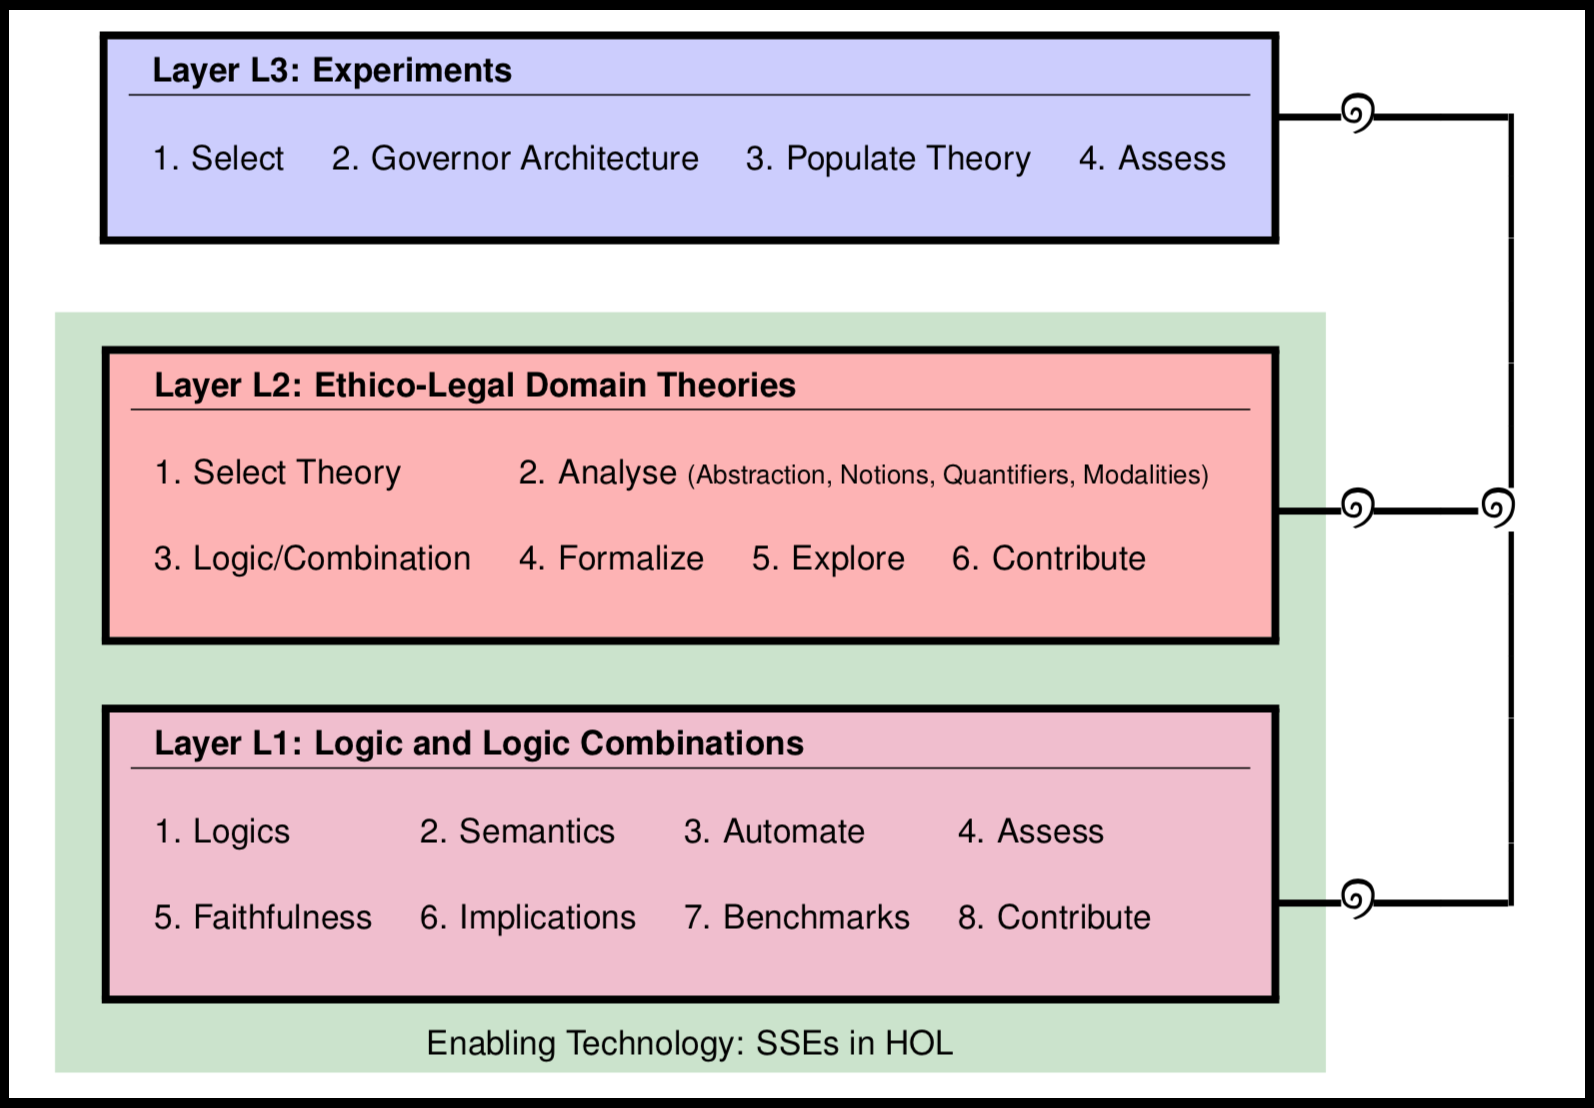
\includegraphics[width=\textwidth]{LogiKEy-methodology.png}
\caption{The LogiKEy logic and knowledge development methodology \label{fig:LogiKEy}}
\end{figure}


\comment{
[Offer a complete description of the experimental design and methods used to acquire these data. Please provide any programs or code files used for filtering and analyzing these data. It is very important that this section is as comprehensive as possible and if you are submitting via another Elsevier journal you are encouraged to provide more detail than in your accompanying research article. There is no character limit for this section, however, no insight, interpretation, or background should be included in this section.]  
}


\subsubsection*{Acknowledgments} We thank all our collaborators and
students from University of Luxembourg and Freie Universit\"at Berlin   
that have already utilized and tested the LogiKEy methodology in several
projects not reported here. 

\subsubsection*{Competing Interests}
Benzm\"uller was funded by the VolkswagenStiftung
  under grant CRAP (Consistent Rational Argumentation in
  Politics). Parent and van der Torre were supported by  the European
  Union's Horizon 2020 research and innovation programme under the
  Marie Sk\l{}odowska-Curie grant agreement MIREL (MIning and
  REasoning with Legal texts) No 690974.

\comment{
[All authors are required to report the following information: 
(1) All third-party financial support for the work this article; 
(2) All financial relationships with any entity that could be viewed as relevant to data described in this manuscript; 
(3) All sources of revenue with relevance to this work where payments have been made to authors, or their institutions on their behalf, within the 36 months prior to submission;
(4) Any other interactions with the sponsors, outside of the submitted work; 
(5) Any relevant patents or copyrights (planned, pending, or issued);
(6) Any other relationships or affiliations that may be perceived by readers to have influenced, or give the appearance of potentially influencing, what has been written in this article. 
As a general guideline, it is usually better to disclose a relationship than not. This information will be acknowledged at publication in the manuscript. If there is no known competing financial interests or personal relationships that could have appeared to influence the work reported in this paper, please include this statement:] 
The authors declare that they have no known competing financial interests or personal relationships which have, or could be perceived to have, influenced the work reported in this article.
[If there are financial interests/personal relationships which may be
considered as potential competing interests, please declare them
here:]
}


%\subsubsection*{References}
\bibliographystyle{abbrv}
\bibliography{Bibliography}

\comment{
[References are limited (approx. 15) and excessive self-citation is not allowed. If your data article is co-submitted via another Elsevier journal, please cite your associated research article here.
Reference style: 
Text: Indicate references by number(s) in square brackets in line with the text. The actual authors can be referred to, but the reference number(s) must always be given. 
Example: '..... as demonstrated [3,6]. Barnaby and Jones [8] obtained a different result ....' 
List: Number the references (numbers in square brackets) in the list in the order in which they appear in the text. 
Examples: 
Reference to a journal publication: 
[1] J. van der Geer, J.A.J. Hanraads, R.A. Lupton, The art of writing a scientific article, J. Sci. Commun. 163 (2010) 51–59. https://doi.org/10.1016/j.Sc.2010.00372.
Reference to a journal publication with an article number: 
[2] Van der Geer, J., Hanraads, J.A.J., Lupton, R.A., 2018. The art of writing a scientific article. Heliyon. 19, e00205. https://doi.org/10.1016/j.heliyon.2018.e00205.
Reference to a book: 
[3] W. Strunk Jr., E.B. White, The Elements of Style, fourth ed., Longman, New York, 2000. 
Reference to a chapter in an edited book: 
[4] G.R. Mettam, L.B. Adams, How to prepare an electronic version of your article, in: B.S. Jones, R.Z. Smith (Eds.), Introduction to the Electronic Age, E-Publishing Inc., New York, 2009, pp. 281–304.
Reference to a website:
[5] Cancer Research UK, Cancer statistics reports for the UK. http://www.cancerresearchuk.org/aboutcancer/statistics/cancerstatsreport/, 2003 (accessed 13 March 2003).
Reference to a dataset:
[6] [dataset] M. Oguro, S. Imahiro, S. Saito, T. Nakashizuka, Mortality data for Japanese oak wilt disease and surrounding forest compositions, Mendeley Data, v1, 2015. https://doi.org/10.17632/xwj98nb39r.1.]
}

\end{document}